350. Раз Георгий проиграл Дмитрию треть игр между ними, всего было 3 игры, 2 из которых он выиграл, то есть игры Георгия и Дмитрия закончились со счётом $2:1,$ а Дмитрия и Георгия --- $1:2.$ Борис проиграл Виктору 3 раза, значит и всем остальным он проиграл по 3 раза, и игры Бориса и Виктора закончились со счётом $1:3,$ Виктора и Бориса $3:1,$ Георгия и Бориса $3:3,$ Бориса и Георгия $3:3.$ Из таблицы определим, что Дмитрий проиграл Виктору 2 раза, а выиграл у него 0 раз, значит игры Виктора и Дмитрия закончились со счётом $2:0,$ а Дмитрия и Виктора со счётом $0:2.$ Виктор выиграл 5 раз, значит игры Виктора и Георгия закончились со счётом $0:7,$ а Георгия и Виктора --- $7:0.$ Дмитрий выиграл 4 раза, значит проиграл он 12 раз, и игры Бориса и Дмитрия закончились со счётом $8:3,$ а Дмитрия и Бориса --- $3:8.$ Таким образом, таблица полностью заполнена.\\
\begin{figure}[ht!]
\center{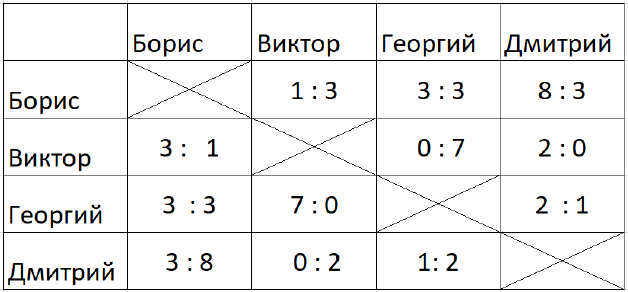
\includegraphics[scale=0.35]{tab1.png}}
\end{figure}\\
